%%%%%%%%%%%%%%%%%%%%%%%%%%%%%%%%%%%%%%%%%%%%%%%%%%%%%%%%%%%%%%%%%%%%%%%%%%%%%
%% 
%% Informal notes on k-randomization.
%% 
%%%%%%%%%%%%%%%%%%%%%%%%%%%%%%%%%%%%%%%%%%%%%%%%%%%%%%%%%%%%%%%%%%%%%%%%%%%%%


\documentclass[11pt]{article}
%\documentclass[11pt,draft]{amsart}

% Custom styling.
\usepackage{custom}
%% Controls enumeration labels
%\usepackage{enumerate}
%% Shrinks margins 
\usepackage{fullpage}
%% Shows equation label keys
%\usepackage[notref]{showkeys}
%% Title matter
\title{Differential privacy in collections of anonymized records}
\author{Maxim Zhilyaev (Apple) and Dave Zeber (Mozilla)}

\usepackage[english]{babel}
\usepackage{graphicx}
\usepackage{booktabs}


%%%%%%%%%%%%%%%%%%%%%%%%%%%%%%%%%%%%%%%%%%%%%%%%%%%%%%%%%%%%%%%%%%%%%%%%%%%%%
\begin{document}
\maketitle

\tableofcontents

\section{Privacy Loss Ratio in anonymized collections}

\subsection{general case - full permutational privacy loss ratio}

Given original database $D$ consisting of $N$  user-records, and synthetic database $S=\{s_1,s_2,s_3, \cdots, s_n\}$ received from $D$ by process of randomization and permutation.
Define $\Pi$ a set of all permutations $\pi(i,j)$ by which one can do bijection from $D$ to $S$.  

In most general formulation, the probability of observing $S$ from a given $D$ has to include both - a probability of generating a particular assortment of synthetic records from corresponding user records and the probability of the permutation itself:

\begin{align}
P(S|D) = \sum_{\pi \in \Pi} \prod_{\begin{matrix} \pi(i,j) \\ u_i \in D \end{matrix}}  p(s_j | u_i) \cdot P[\pi(i,j)]
\end{align}

We now let one of the user records to change. Without loss of generality, we exchange $u_1$ to $u_0$ to receive a neighboring database $D_m$, with corresponding conditional probability of generating  same $S$:
\begin{align}
P(S|D_m) = \sum_{\pi \in \Pi}  \prod_{\begin{matrix} \pi(i,j) \\ u_i \in D_m \end{matrix}}   p(s_j | u_i) \cdot P[\pi(i,j)]
\end{align}

The privacy loss ratio $R(S)$ take the form:

\begin{equation} \label{eq:totalPLR}
R(S) = \frac{P(S|D)}{ P(S|D_m)} = \frac{\sum_{\pi \in \Pi} \prod_{\begin{matrix} \pi(i,j) \\ u_i \in D \end{matrix}}  p(s_j | u_i) \cdot P[\pi(i,j)]} { \sum_{\pi \in \Pi}  \prod_{\begin{matrix} \pi(i,j) \\ u_i \in D_m \end{matrix}}   p(s_j | u_i) \cdot P[\pi(i,j)]}
\end{equation}

Presence of permutational probabilities in  \eqref{eq:totalPLR}  corresponds to various attacks that an observer may lunch on randomized data if it's not sufficiently permuted.   For a really nasty example, suppose that $u_1$ submits his randomized record at midnight and all the rest submit their data at noon, a permutation that maps $u_1$ to any $s$ other then $s_1$ is impossible, and the privacy loss ratio degenerates to a local DP formulation:

\begin{align}
R(S) = \frac{P(S|D)}{ P(S|D_m)} = \frac{p(s_1|u_1) \cdot P(S \cap s_1 | D \cap u_1)}  {p(s_1|u_0)  \cdot P(S \cap s_1 | D \cap u_0) } = \frac{p(s_1|u_1)}{p(s_1|u_0)}
\end{align}


\subsection{privacy loss ratio for equally likely permutations}

We now consider an important case when all permutations are equally likely.  This amounts to inability of an observer to discover any positional correlation between $s_j$ and $u_i$.  If the randomized record from $u_i$ can take any positional index in $S$ with equal probability, then every bijection of $D$ into $S$ is equally likely and cancel each other out in \eqref{eq:totalPLR}, giving  a simplified version of privacy loss ratio:

\begin{equation} \label{eq:mainPLR} 
R(S) =  \frac{P(S|D)}{ P(S|D_m)}  = \frac{\sum_{\pi \in \Pi} \prod_{\begin{matrix} \pi(i,j) \\ u_i \in D \end{matrix}}  p(s_j | u_i) } { \sum_{\pi \in \Pi}  \prod_{\begin{matrix} \pi(i,j) \\ u_i \in D_m \end{matrix}}   p(s_j | u_i) }
\end{equation}

It's easy to guarantee uniformly random permutation if a dataset is released by an owner to the observer, in which case a random permutter simply shuffles randomized records of the original dataset before releasing them.  A more complicated setup happens when user devices report their records independently.  Unless measures are taken, an observer can find correlations between time of arrival and user audience:  Chinese audience mostly report at midnight UTC, while US audience most reports noon UTC.  This an undesirable affect - an observer should not gain any insight into the nature of a record by time of its arrival.  To deflect such attack, individual device records are channeled through \href{https://leastauthority.com/blog/mixnet-intro/}{mix-network} with uniformly random delays.  As a result, a record sent by a device arrives anytime with 24 hours of submission, which establishes the claim of "equally likely permutations".  Security procedures that allow a user to establish a trust into anonymization of his records are available: a user (including the observer of the synthetic data) can independently verify the time-randomness of data submissions.  The embodiment of such such procedure is outside the scope of this document and will be presented elsewhere.  For now we assume, a user report is delayed randomly enough to make an observer choose uniform distribution for $D$ to $S$ bijections.


\subsection{privacy loss ratio in datasets with an outlier}

We now consider a fundamental use case when the record $u_1$ is an  \textbf{outlier}  in $D$.  That is $D_m$ consists of identical records $u$ different from $u_1$.  We study the privacy loss ratio and develop important properties of such setup with respect to $(\epsilon, \delta)$ DP formalism.

\begin{defn}
$U_K$ - a collection of $K$ identical records $u$
\end{defn}

Expressing the neighboring dataset sets with the aim of the definition above gives:
\begin{align}
D = U_N  \\
D_m = U_{N-1} \cup u_1
\end{align}

Since all records in $D$ are identical, then every permutation is equal to $\prod_{j=1}^N p(s_j | u)$ and $P(S|D)$ simplifies to:

\begin{align}
P(S|D) = P(S|U_N) = \sum_{\pi \in \Pi}  \prod_{\pi(i,j)}   p(s_j | u) = N!   \prod_{j=1}^N p(s_j | u) 
\end{align}

Now, $D_m$ has one record $u_1$ different from the remaining $N-1$ identical records $u$.  Conditioning of $P(S|D_m)$ provides the following expression:
\begin{align}
P(S|D_m) =  P(S|U_{N-1} \cup u_1) = p(s_1|u_1) P(S \cap s_1 | U_{N-1}) + \cdots  + p(s_N|u_1) P(S \cap s_N | U_{N-1}) \\
= \sum_{i=1}^N p(s_i | u_1) P(S \cap s_i | U_{N-1})
\end{align}

The probability $ P(S \cap s_i | U_{N-1})$ can be expressed as:

\begin{align}
P(S \cap s_i | U_{N-1})=   (N-1)! \prod_{j=1, j \ne i}^N p(s_j | u) 
\end{align}

From here we can express privacy loss ratio for $S$     

\begin{align}
R(S) =  \frac{P(S|D)}{ P(S|D_m)}  = \frac{ P(S|U_N)} {P(S|U_{N-1} \cup u_1)} \\
= \frac  {  N!   \prod_{j=1}^N p(s_j | u)  }{ \sum_{i=1}^N p(s_i | u_1)   (N-1)! \prod_{j=1, j \ne i}^N p(s_j | u)  } \\
=  N / \left ( \sum_{i=1}^N p(s_i | u_1) \frac {  \prod_{j=1, j \ne i}^N p(s_j | u)  } {  \prod_{j=1}^N p(s_j | u)  } \right )\\
=    \frac{N}{\sum_{i=1}^N  \frac{ p(s_i | u_1) } { p(s_i | u) }}
\end{align}

Restating for clarity:
\begin{equation} \label{eq:outlierPLR} 
R(S) =  \frac{P(S|D)}{ P(S|D_m)}  = \frac{ P(S|U_N)} {P(S|U_{N-1} \cup u_1)} = \frac{N}{\sum_{i=1}^N  \frac{ p(s_i | u_1) } { p(s_i | u) }}
\end{equation}

And an important consequence of this relation:
\begin{equation} \label{eq:outlierProbs} 
P(S|U_{N-1} \cup u_1) =  P(S|U_N)  \frac{\sum_{i=1}^N  \frac{ p(s_i | u_1) } { p(s_i | u) }}{N}
\end{equation}

$(\epsilon, \delta)$ DP requires that both $R(S)$ and it's reciprocal are bounded by $e^{\epsilon}$ with the probability $1-\delta$.
\begin{align}
P(R(S) < e^{\epsilon} ) \le 1 - \delta \\ 
P(\frac{1}{R(S)} <  e^{\epsilon} ) \le 1 - \delta
\end{align}

Which bounds we will develop in the subsequent sections

\subsection{Outlier absence vs. presence privacy loss}

Note in the sum $\sum_{i=1}^N  \frac{ p(s_i | u_1) } { p(s_i | u) }$ in the denominator of $R(S)$ is just the sum of privacy loss ratios of each individual synthetic record.  However the value of this sum crucially depends on the underling distribution of $S$.  This is a subtle (but fundamental) issue so we spend some time on it.  Consider the $R(S)$ again.
\begin{equation} \label{eq:outlierPLR} 
R(S) =  \frac{ P(S|U_N)} {P(S|U_{N-1} \cup u_1)} = \frac{N}{\sum_{i=1}^N  \frac{ p(s_i | u_1) } { p(s_i | u) }}
\end{equation}

This ratio measures privacy loss when $S$ is generated from $U_N$, and quantifies the ease with which an observer can tell the presence or absence of record $u_1$ provided the synthetic output is generated from $U_N$.  In other words, should the synthetic output come from $U_N$ we want its outlier neighbor $U_{N-1} \cup u_1$ be DP-indistinguishable: and so we \textbf{let $U_N$ generate various incarnations of $S$} and bound how small the sum $\sum_{i=1}^N  \frac{ p(s_i | u_1) } { p(s_i | u) }$ can get for an arbitrary $S$ provided it comes from $U_N$. 

Now let's revert the privacy ratio to its reciprocal which also has to meet $(\epsilon, \delta)$ DP bounds:
\begin{align}
\frac{1}{R(S)} =   \frac {P(S|U_{N-1} \cup u_1)} { P(S|U_N)} = \frac{1}{N} \sum_{i=1}^N  \frac{ p(s_i | u_1) } { p(s_i | u) }
\end{align}

It is the exact same sum, but the distribution of $S$ radically changes.  Now $S$ is generated by $U_{N-1} \cup u_1$ and so we want to make sure that its neighbor $U_N$ is  DP-indistinguishable.  In another word, if there's truly an outlier we want to have enough noise to hide it (that is, make it DP-indistinguishable from the dataset  $U_N$ that has no outlier), and so we \textbf{let $U_N \cup u_1$ generate various incarnations of $S$} and bound how high of sum $\sum_{i=1}^N  \frac{ p(s_i | u_1) } { p(s_i | u) }$ can get for an arbitrary $S$ provided it comes from $U_N \cup u_1$.

There is a distributional asymmetry that we have to account for when dealing with the sum $\sum_{i=1}^N  \frac{ p(s_i | u_1) } { p(s_i | u) }$.  Hence, we define the following quantities to help keep track of dataset that generates $S$.


\textbf{Definition}
\begin{itemize}
\item $\mathbb{X}_N(D) = \sum_N  \frac{ p(s_i | u_1) } { p(s_i | u)}$ is a random variable representing the sum computed over $S$ generated from dataset $D$.
\item $\bar{\mathbb{X}}_N(D) = \frac{\sum_N  \frac{ p(s_i | u_1) } { p(s_i | u)} }{N}$ - a mean of the sum computed over $S$ generated from dataset $D$.
\end{itemize}

Furthermore, there are two semantically different privacy loss ratios - one is $R(S)$ which attempts to hide the \textbf{absence} of an outlier: that is  we want an outlier dataset  $U_{N-1} \cup u_1$ be indistinguishable from  no-outlier dataset $U_N$ on the output that $U_N$ generates.  We shall call this ratio the \textbf{outlier absence privacy loss}.   The other ratio is semantically opposite - we want the no-outlier dataset $U_N$ be indistinguishable from an outlier dataset  $U_{N-1} \cup u_1$ on the output  $U_{N-1} \cup u_1$ generates, and we shall call this ratio \textbf{outlier presence privacy loss}.

In what follows we demonstrate that
\begin{itemize}
\item bounding \textbf{outlier absence ratio} also bounds  \textbf{outlier presence ratio}, hence \textbf{outlier absence ratio} is the largest of two
\item either kind of ratio maximizes when the neighboring dataset are $U_N$ and  $U_N \cup u_1$, that is these two data sets from a maximally revealing pair of neighboring datasets. 
\end{itemize}

\section{Distributional properties of  $\mathbb{X}_N(U_N)$}  

When synthetic output is generated from $U_N$ the probability of generating a particular value of $s$ depends only on $u$, meaning that the sum  $\mathbb{X}_N(U_N) = \sum_N  \frac{ p(s_i | u_1) } { p(s_i | u)}$ degenerates to the sum of i.d.d. random variables $\frac{ p(s | u_1) } { p(s | u)}$ where $s$ is a synthetic output of $u$.  As we show later moments of the same sum generated from datasets other then $U_N$ can be computed from moments of $\mathbb{X}_N(U_N)$, hence we spend some time developing tools that describe how  $\mathbb{X}_N(U_N)$ is distributed.

\textbf{Definition}
\begin{itemize}
\item $X_u = \frac{p(s | u_1) } { p(s| u)}$ is a random variable representing privacy loss ratio between records $u_1$ and $u$ when $s$ comes from $u$
\item $\mathbb{X}_N = \sum_N X_u$ is a random variable representing the sum of $N$ i.d.d random variables $X_u$
\item $\bar{\mathbb{X}}_N = \frac{\sum_N X_u}{N}$ - a sampling mean from $X_u$
\end{itemize}

 The underling distribution of $X_u$ is defined on a set $\Omega$ of all possible synthetic records $s$, and it's easy to see that $E(X_u)$ is always 1.
\begin{align}
E(X_u) = \sum_{s \in \Omega}   \frac{p(s | u_1) } { p(s| u)} \cdot p(s|u) = \sum_{s \in \Omega} p(s|u_1) = 1
\end{align}

Let's define yet another random variable $X_1 = \frac{p(s|u_1)}{p(s|u)}$ when $s$ is generated by $u_1$ and show how moments of both distributions are related. 

\begin{lem}
k-th moment of $X_u$ is equal to $k-1$ moment of $X_1$
\end{lem}
 
 Proof:
 Let $s$ takes values in domain $\Omega$, then a k-th moment of $X_u$ is written as:
 \begin{align}
M_k(X_u) =  \sum_{s \in \Omega} \left [ \frac{p(s|u_1)}{p(s|u)} \right ]^k \cdot p(s|u) =  \sum_{s \in \Omega} \left [ \frac{p(s|u_1)}{p(s|u)} \right ]^{k-1} \cdot  \frac{p(s|u_1)}{p(s|u)} \cdot p(s|u) \\
=  \sum_{s \in \Omega} \left [ \frac{p(s|u_1)}{p(s|u)} \right ]^{k-1} \cdot  p(s|u_1) = M_{k-1}(X_1) 
 \end{align}
 
 \subsection{Renyi divergence}
 
Renyi divergence proved invaluable tool for extracting distributional parameters of $X_u$ and $X_1$ for the whole spectra of use cases and techniques.  We shall focus on applications when reported records are bit vectors, but the case for continues real values is handled similarly.   For exhaustive list of properties see \href{https://arxiv.org/pdf/1206.2459.pdf}{Renyi Divergence and Kullback-Leibler Divergence}
 
Consider Renyi divergence between distributions $P(s|u_1)$ - a distribution of $X_1$, and $Q(s|u)$ - a distribution of $X_u$.
\begin{align}
D_{\alpha} (P \parallel Q ) = \frac{1}{\alpha - 1} \log \left [ \sum_{s \in \Omega} \frac{P(s|u_1)^{\alpha}}{ Q(s|u)^{\alpha-1} } \right ] =  \frac{1}{\alpha - 1} \log \left [ \sum_{s \in \Omega} \frac{p(s|u_1)^{\alpha}}{ p(s|u)^{\alpha-1} } \right ] 
\end{align}

\begin{lem}
Renyi divergence generates log of moments $M_k(X_1)$ when $\alpha = k+1$
\end{lem}
\begin{pf}

Since $X_1 =   \frac{p(s|u_1)}{p(s|u)}$  where $s$ is generated by $u_1$, we have
\begin{align}
D_{\alpha} (P \parallel Q ) =   \frac{1}{\alpha - 1} \log \sum_{s \in \Omega} \frac{p(s|u_1)^{\alpha}}{ p(s|u)^{\alpha-1} } \\
= \frac{1}{\alpha-1} \log \left [ \sum_{s \in \Omega} p(s|u_1) \frac{p(s|u_1)^{\alpha-1}}{ p(s|u)^{\alpha-1} } \right ] \\
=   \frac{1}{\alpha-1} \log \left [ E \left ( \frac{p(s|u_1)^{\alpha-1}}{ p(s|u)^{\alpha-1} } \right ) \right ] \\
=  \frac{1}{\alpha-1} \log [M_{\alpha-1}(X_1)] 
\end{align}
\end{pf}

The immediate consequence of this are expressions for mean and variance of $X_1$
 \begin{align}
 D_2 (P \parallel Q )  =  log [M_{1}(X_1)] = log[ E(X_1) ] \\
 D_3 (P \parallel Q )  = \frac{1}{2} log [M_{2}(X_1)] = \frac{1}{2} log[ E(X_1^2) ]
 \end{align}

Another useful property of Renyi divergence is that divergence of the product distributions is a sum of divergences for individual distributions of the product, which we can apply to the composite records.  Suppose  $u_1$ and $u$ consist of $L$ independent parts, and each part is subjected to randomization independently.  Then distributions $P$ and $Q$ become product of the distributions of each part.  Having $i$ be the index of the individual part, and $u(i)$ and $s(i)$ be the respective $i-th$ values of real and synthetic records, one can write:
 \begin{align}
 P(s|u_1) = \prod_{i}^L p_i(s(i) | u_1(i))  \\
 Q(s|u) =  \prod_{i}^L p_i(s(i) | u(i)) 
\end{align}

Using the property above we can conveniently express Renyi divergence of a composite record through divergencies of its parts.

\begin{equation}  \label{eq:divergBits} 
 D_{\alpha} (P \parallel Q ) =  \sum_i^L  D_{\alpha} (P_i \parallel Q_i) =  \frac{1}{\alpha - 1} \log \prod_{i}^L  M_{\alpha-1}(X_1(i))
\end{equation}

Where $X_1(i)$ is the random variable $X_1$ corresponding to $i-th$ part.

We shall use these results extensively for computing moments of $X_1$ (and $X_u$) for various randomization mechanisms and their mixes.

\subsection{maximal outlier}
 \begin{defn}
A maximal outlier $u_1$ with respect to $u$ is a record that maximizes  $\frac{ p(s | u_1) } { p(s| u) }$ for the same amount of noise.  
\end{defn}

It follows from the form of Renyi divergence that moments of $X_1$ (and $X_u$) are maximized when the function bellow is maximized:
\begin{align}
\sum_{s \in \Omega} p(s|u_1) \frac{p(s|u_1)^{\alpha-1}}{ p(s|u)^{\alpha-1} }
\end{align}
which happens when $u_1$ is chosen as different from $u$ as possible.  For the randomization mechanism studied in this paper, $u_1$ is always the a record maximally distant from $u$ according to some distance measure.  For example, if the records are taking the form of bit vectors, the maximal outlier $u_1$ has the largest Humming distance from $u$, that is it's different from $u$ in every bit.  One can easily see why from the corresponding Renyi divergence for bit vectors, which maximizes when bits between $u_1$ and $u$ are indeed different in every position. Same is holding for continuous types of randomization mechanism such as Laplacian or Normal noise.  Once can show that $E(X_1)$ reaches maximum for noise parameters of a given mechanism if Euclidean distance between $u_1$ and $u$ is the largest.  Thereafter we assume that $u_1$ is a maximal outlier with respect to identical records records $u$ that compose the dataset $U_N$.  

The important property of the maximal outlier is that corresponding moments are maximized, which implied that we only need to privacy bound the neighboring datasets $U_N$ and $U_{N-1} \cup u_1$ when $u_1$ is maximal outlier.  All the remaining cases will have lesser variances and, therefore, will be bound by the same noise level.

\section{Bounding privacy loss ratio}

\subsection{outlier absence privacy loss bounds}

The privacy loss bound for this case is:
\begin{align}
P(R(S) < e^{\epsilon} ) \le 1 - \delta \\ 
\end{align}

Setting $\lambda = e^{\epsilon}$ for connivence, we have:
 
 \begin{align}
R(S) =  \frac{N}{\sum_N  \frac{ p(s | u_1) } { p(s | u) }}  \le  \lambda \\
\frac{1}{\bar{\mathbb{X}}_N} \le \lambda \\
\bar{\mathbb{X}}_N = \frac{\sum_N X_u}{N} \ge \frac{1}{\lambda}
\end{align}

Note that $\bar{\mathbb{X}}_N$ is a sampling mean from $X_u$ and, therefore, distributed normally according to CLT.   Hence, we simply need to low bound a normal distribution with known mean and deviation:

\begin{align}
P \left (\frac{ \sum_N X_u}{N} <  \frac{1}{\lambda} \right ) = P  \left (  \mathbb{N} \left ( 1, \sqrt{\frac{\var(X_u)}{N})} \right ) \le   \frac{1}{\lambda} \right ) \le \delta
\end{align}

Then to ensure $\delta$ bound is met, we choose  a multiple of deviations $\beta$ so that  the probability of observing $\bar{\mathbb{X}}_N$ above $1 -  \beta \cdot \sigma$ is small:
\begin{align}
P (\bar{\mathbb{X}}_N > 1 - \beta \cdot \sigma) \le \delta
\end{align}

And then for given $\beta$ we low bound  $\bar{\mathbb{X}}_N$  to fit the privacy loss ratio limit

\begin{align}
1 - \beta \cdot \sigma \ge  \frac{1}{\lambda} \\
 \beta \cdot \sigma \le 1 -  \frac{1}{\lambda} \\
\sigma \le \frac{\lambda - 1}{\beta\lambda} \\
\var(X_u) \le N \left ( \frac{\lambda - 1}{\beta\lambda} \right )^2 \\
\end{align}

The last expression allows to extract the smallest allowed noise parameter from the expression of the variance of the randomization mechanism at hand. 

 \subsection{outlier presence privacy loss bounds}

Recall that outlier presence privacy loss ratio is computed on $S$ generated from $U_{N-1} \cup u_1$:
\begin{align}
\frac{1}{R(S)} =  \frac{\mathbb{X}_N(U_{N-1} \cup u_1)}{N} = \bar{\mathbb{X}}_N(U_{N-1} \cup u_1)
\end{align}

From \eqref{eq:outlierProbs}  we have 
\begin{align}
P(S|U_{N-1} \cup u_1) =  P(S|U_N)  \frac{\sum_N  \frac{ p(s | u_1)} { p(s | u) }}{N} 
\end{align}

\begin{lem}
k-th moment of $\frac{1}{R(S)}$ is equal to $k+1$ moment of $R(S)$, and $\frac{1}{R(S)}$ is a sampling mean of $X_1$ (which is a distribution of  ratio $\frac{ p(s | u_1)} { p(s | u) }$ when $s$ is generated from $u_1$)
\end{lem}
Proof:
\begin{align}
\sum  \bar{\mathbb{X}}_N^k(U_{N-1} \cup u_1) \cdot P(S|U_{N-1} \cup u_1) \\
= \sum \left ( \frac{\sum_N  \frac{ p(s | u_1)} { p(s | u) }}{N}  \right )^k  \cdot P(S|U_{N-1} \cup u_1) \\
=  \sum \left ( \frac{\sum_N  \frac{ p(s | u_1)} { p(s | u) }}{N}  \right )^k \cdot  \frac{\sum_{s \in \Omega}  \frac{ p(s | u_1)} { p(s | u) }}{N}  \cdot P(S|U_N) \\
= \sum \left ( \frac{\sum_N  \frac{ p(s | u_1)} { p(s | u) }}{N}  \right )^{k+1} \cdot P(S|U_N)
\end{align}

Since $R(S)$ is sampling mean of $X_u$, and $k$ moment of $X_1$ is equal to $k+1$ moment of $X_u$, then  $\frac{1}{R(S)}$ is a sampling mean from $X_1$ by uniqueness of the moment generation function. That is the distribution of $\bar{\mathbb{X}}_N(U_{N-1} \cup u_1)$ is a sampling mean form $X_1$.  

We now can upper bound $1/R(S)$ by limiting deviation of a sampling mean of $X_1$.

To ensure $\delta$ bound is met,  choose a multiple of deviations $\beta$ so that  the probability of observing $\bar{\mathbb{X}}_N(U_{N-1} \cup u_1)$ above $1+  \beta \cdot \sigma$ is small:
\begin{align}
P (\bar{\mathbb{X}}_N(U_{N-1} \cup u_1) > 1 + \beta \cdot \sigma) \le \delta
\end{align}

Then for given $\beta$ bound the privacy loss ratio $1/R(S)$:
\begin{align}
\bar{\mathbb{X}}_N(U_{N-1} \cup u_1) \le \lambda \\
\frac{E(X_1) }{N}+ \beta \cdot \sigma \le \lambda \\
\sigma \le \frac{\lambda - \frac{E(X_1)}{N}}{\beta} \\
\sqrt{\frac{\var(X_1)}{N}} \le \frac{\lambda - \frac{E(X_1)}{N}}{\beta} \\
\var(X_1) \le N \left ( \frac{\lambda - \frac{E(X_1)}{N}}{\beta} \right )^2 \\
\end{align}

Then solve the above inequality numerically to find maximal amount of noise sufficient to satisfy the bound.  

\subsection{Outlier absence privacy loss is larger than outlier presence privacy loss}

In this section we show that bounding $R(S)$ also bounds $\frac{1}{R(S)}$.  In other words, the noise needed to hide the outlier absence is enough to hide the outlier presence. 

Recall that bounding outlier absence privacy loss amounts to establishing DP inequality when synthetic output is generated from $U_N$.
\begin{align}
\bar{\mathbb{X}}_N = \frac{\sum_N  \frac{ p(s | u_1) } { p(s | u) }}{N}  \\
 P \left ( \bar{\mathbb{X}}_N  \ge  \frac{1}{\lambda} \bigg | U_N \right) \ge \delta
 \end{align}

Then the low bound $\bar{\mathbb{X}}_N \ge \frac{1}{\lambda}$ holds for any synthetic output $S$ with probability $P(S|U_N) \ge \delta$.

Using \eqref{eq:outlierProbs} we deduce the following:
\begin{align}
P\left ( \bar{\mathbb{X}}_N \ge \frac{1}{\lambda}  \bigg | U_N \right) \ge \delta \text{ , therefore }\\
P\left ( \bar{\mathbb{X}}_N \ge \frac{1}{\lambda}  \bigg | U_{N-1} \cup u_1 \right)  = \bar{\mathbb{X}}_N P\left ( \bar{\mathbb{X}}_N \ge \frac{1}{\lambda}  \bigg | U_N \right)  \ge  \frac{P\left ( \bar{\mathbb{X}}_N \ge \frac{1}{\lambda}  \bigg | U_N \right) }{\lambda}  \ge \frac{ \delta}{ \lambda} \ge \delta
 \end{align}
 
 The other side of the bound is more involved.  Note that when $ \bar{\mathbb{X}}_N$ reaches $\lambda$, the probability of $U_{N-1} \cup u_1$ generating its corresponding values is again given by  \eqref{eq:outlierProbs}:
\begin{align}
P \left( \bar{\mathbb{X}}_N \le \lambda |  U_{N-1} \cup u_1 \right)  =  \bar{\mathbb{X}}_N P \left( \bar{\mathbb{X}}_N \le \lambda |  U_N \right) \le \lambda P \left( \bar{\mathbb{X}}_N \le \lambda |  U_N \right)
\end{align}

Since we bounded $\sigma$ of $\bar{\mathbb{X}}_N$ distribution to
\begin{align}
\sigma \le \frac{\lambda - 1}{\beta \lambda}
\end{align}

Then at $\lambda$ the $\bar{\mathbb{X}}_N$ will $\beta \cdot \lambda$ deviations from its mean.
\begin{align}
E(\bar{\mathbb{X}}_N (U_N)) = 1 \\
\frac{(\lambda - E(\bar{\mathbb{X}}_N (U_N))}{\sigma} = \frac{\lambda - 1}{\sigma} = \beta \cdot \lambda
\end{align}

$\beta$ was chosen to bound:
\begin{align}
P(\bar{\mathbb{X}}_N < 1 - \beta \sigma) \le \delta
\end{align}

And it follows from the symmetry of the distribution around the mean that
\begin{align}
P(\bar{\mathbb{X}}_N > 1 + \beta \sigma) \le \delta
\end{align}

From here, we need to prove that 
\begin{align}
\lambda \cdot P(\bar{\mathbb{X}}_N > 1 +  \lambda \beta \sigma) \le \delta
\end{align}

\textbf{@TBD}
On the surface it follows from the fact that normal probability drops exponentially as we deviate away from mean, which can't be compensated by linear increase.   There is good bound here: https://math.stackexchange.com/questions/74760/bounds-on-normal-distribution that I think is applicable for the proof.  Skipping this step as it's purely technical - we can prove it later.

\section{Maximality proofs}

\subsection{Maximality of outlier absence privacy loss}

In this section we show why outlier absence privacy loss maximizes in dataset $U_N$.  Consider neighboring pair of datasets that contains yet another record $u'$ potentially different from either $u_1$ or $u$.  We are still replacing $u$ with it's maximal outlier $u_1$, hence
\begin{align}
D' = U_{N-1} \cup u' \\
D'_m =  U_{N-2} \cup u' \cup u_1
\end{align}

The probability $P(S|D)$ comes from \eqref{eq:outlierProbs} :
\begin{align}
P(S|D) = P(S|U_{N-1} \cup u') =  P(S|U_N)  \frac{\sum_N  \frac{ p(s | u') } { p(s | u) }}{N}
\end{align}

The probability of $P(S|D'_m)$ take the form below:
 \begin{equation}  
P(S|D'_m) = P(S'|U_{N-2} \cup u_1 \cup u' ) =  \frac{P(S|U_{N})}{N(N-1)} \cdot \left (  \sum_N  \frac{ p(s | u') } { p(s | u) } \cdot  \sum_N \frac{ p(s | u_1) } { p(s | u)}   - \sum_N  \frac{ p(s | u') } { p(s | u) } \cdot \frac{ p(s | u_1) } { p(s | u)}  \right )
\end{equation}

Derivation of this expression is involved and was moved to Appendix 1.

From the formula above, we establish an expression for privacy loss ratio in the presence of a single foreign record $u'$:
\begin{align}
R'(S) = \frac{P(S|U_{N-1} \cup u')}{P(S|U_{N-2} \cup u' \cup u_1 )} = \frac{ (N-1)  \sum_N  \frac{ p(s | u') } { p(s | u) } } 
{ \sum_N  \frac{ p(s | u') } { p(s | u) } \cdot  \sum_N \frac{ p(s | u_1) } { p(s | u)}   - \sum_N  \frac{ p(s | u') } { p(s | u) } \cdot \frac{ p(s | u_1) } { p(s | u)}  }
\end{align}

Let's bound $R'(S)$ to be less than $\lambda$
\begin{align}
\frac{ (N-1)  \sum_N  \frac{ p(s | u') } { p(s | u) } } 
{  \sum_N  \frac{ p(s | u') } { p(s | u) } \cdot  \sum_N \frac{ p(s | u_1) } { p(s | u)}   - \sum_N  \frac{ p(s | u') } { p(s | u) } \cdot \frac{ p(s | u_1) } { p(s | u)}   }  \le \lambda \\
\frac {\sum_N  \frac{ p(s | u') } { p(s | u) } \cdot  \sum_N \frac{ p(s | u_1) } { p(s | u)}   - \sum_N  \frac{ p(s | u') } { p(s | u) } \cdot \frac{ p(s | u_1) } { p(s | u)}   }  { (N-1)  \sum_N  \frac{ p(s | u') } { p(s | u) } }  \ge \frac{1}{\lambda} \\
\sum_N \frac{ p(s | u_1) } { p(s | u)}   - \frac{ \sum_N  \frac{ p(s | u') } { p(s | u) } \cdot \frac{ p(s | u_1) } { p(s | u)}  }  {  \sum_N  \frac{ p(s | u') } { p(s | u) } }  \ge \frac{N-1}{\lambda} 
\end{align}

It can be shown (see Appendix 3)  that
\begin{align}
\frac{ \sum_N  \frac{ p(s | u') } { p(s | u) } \cdot \frac{ p(s | u_1) } { p(s | u)}  }  {  \sum_N  \frac{ p(s | u') } { p(s | u) } }  =  \frac{\sum_N \frac{ p(s | u_1) } { p(s | u)}}{N}
\end{align}

Then
\begin{align}
\sum_N \frac{ p(s | u_1) } { p(s | u)}   - \frac{ \sum_N  \frac{ p(s | u') } { p(s | u) } \cdot \frac{ p(s | u_1) } { p(s | u)}  }  {  \sum_N  \frac{ p(s | u') } { p(s | u) } }  \ge \frac{N-1}{\lambda}  \\
\sum_N \frac{ p(s | u_1) } { p(s | u)}   -  \frac{\sum_N \frac{ p(s | u_1) } { p(s | u)}}{N}  \ge \frac{N-1}{\lambda}  \\
\frac{(N-1)\sum_N \frac{ p(s | u_1) } { p(s | u)}}{N}  \ge \frac{N-1}{\lambda}  \\
\frac{\sum_N \frac{ p(s | u_1) } { p(s | u)}}{N}  \ge \frac{1}{\lambda} \\
\frac{\mathbb{X}_N(U_{N-1} \cup u')}{N} \ge \frac{1}{\lambda} 
\end{align}

\textbf{@TBD} proving above should be pretty much the same proof as in \textbf{3.32}

\subsection{Maximality of outlier presence privacy loss}
\textbf{@TBD}  

\section{Utility of Randomization methods under anonymization}
In this section we put the theory developed above to work and show how significant the gain anonymization provides in terms of reducing required DP noise and boosting the precision of the measurements.  We focus on two main use cases:  RRT - a bit flipping randomization, and Laplacian noise mechanism applied to a continuous variable.  Of cause, both types of data can be combined in a user record, and both types of randomization can applied to corresponding parts of that record. Due to the composition property of Renyi  divergence exact same methodology is applicable to records containing a mixture of data with different types. 

As we exemplify different use cases, the methodology remains the same:
\begin{itemize}
\item determine maximally different pair of individual records $u$ and $u_1$
\item compute central moments of $X_1$ using Renyi divergence
\item bind the outlier presence privacy loss $\frac{\sum_N X_1}{N}$ to meet $(\epsilon, \delta)$ DP bounds
\item extract lowest noise parameter from DP bounds
\item compute measurement error (deviation of the estimate) of corresponding measurement estimates
\item compare measurement error to that of local DP
\end{itemize} 

\subsection{Bit flipping randomization (i.e. RRT method)}
Suppose records are bit vectors of length $L$.  The bit flipping randomization proceeds in the following way: each bit of every original bit vector is flipped with probability $q$ and left the same with probability $p=1-q$.  This mechanism's  noise parameter is $q$ - frequency with which bits of an original vector are flipped to receive  a synthetic vector $s$.  

Maximally distant records $u$ and $u_1$ are simply bit vectors different from each other in every bit. Central moments of $X_1$ are readily available from the application Reni convergence theorem \eqref{eq:divergBits} .
  \begin{align*}
  D_{\alpha} (X_1) =   \frac{1}{\alpha - 1} \log \prod_{i}^L \left (  \frac{p(0|u_1(i))^{\alpha}}{ p(0|u(i))^{\alpha-1} } +   \frac{p(1|u_1(i))^{\alpha}}{ p(1|u(i))^{\alpha-1} } \right )
 \end{align*}

 For a single bit position the corresponding bit-wise divergence becomes:
 \begin{align*}
 \frac{p(0|1)^{\alpha}}{ p(0|0)^{\alpha-1} } +   \frac{p(1|1)^{\alpha}}{ p(1|0)^{\alpha-1} } =  \frac{q^{\alpha}}{ p^{\alpha-1} } +   \frac{p^{\alpha}}{ q^{\alpha-1} } = \frac{q^{2\alpha -1} + p^{2\alpha -1}}{ (pq)^{\alpha-1}}
 \end{align*}

 And since original vectors differ in every position, the resulting divergence and moments of $X_1$ take the forms below:
   \begin{align*}
  D_{\alpha} (X_1) =   \frac{1}{\alpha - 1} \log \prod_{i}^L \left (  \frac{q^{2\alpha -1} + p^{2\alpha -1}}{ (pq)^{\alpha-1}} \right ) =  \frac{1}{\alpha - 1} \log \left (  \frac{q^{2\alpha -1} + p^{2\alpha -1}}{ (pq)^{\alpha-1}} \right )^L  \\
  M_{\alpha-1} (X_1) =  \left (  \frac{q^{2\alpha -1} + p^{2\alpha -1}}{ (pq)^{\alpha-1}} \right )^L
 \end{align*}

 From here we extract central moments of of $X_1$:
  \begin{align*}
 E(X_1) =  \left ( \frac{q^3 + p^3}{ pq } \right )^L \\
 E(X_1^2) =  \left ( \frac{q^5 + p^5}{ (pq)^2 } \right )^L \\
VAR(X_1) =  \left ( \frac{q^5 + p^5}{ (pq)^2 } \right )^L - \left ( \frac{q^3 + p^3}{ pq } \right )^{2L}
\end{align*}

Recall that the outlier presence privacy loss bound is met when the inequality below holds:
\begin{align}
\var(X_1) \le N \left ( \frac{\lambda - \frac{E(X_1)}{N}}{\beta} \right )^2
\end{align}

Where $\lambda = e^{\epsilon}$ and $\beta$ is the number of deviations that guarantees the probability of standard normal variable being $\beta$ falls below $\delta$.  For practical purposes setting $\beta=3$ seems reasonable as it corresponds to $\delta=0.001$ - arguably low enough to provide adequate privacy.

Using bounding formula for bit flipping moments we get:
\begin{align}
 \left ( \frac{q^5 + p^5}{ (pq)^2 } \right )^L - \left ( \frac{q^3 + p^3}{ pq } \right )^{2L} \le N \left ( \frac{\lambda - \frac{  \left ( \frac{q^3 + p^3}{ pq } \right )^L }{N}}{\beta} \right )^2
\end{align}

This inequality can be solved numerically for concrete values of parameters.

\subsubsection{Precision gain of bit flipping randomization}

Suppose that the original dataset consists only of indicator bit vectors, each having exactly one set bit, and that the bit in position $j$ is set for $d$ out of the $N$ vectors.
The number $M$ of synthetic vectors (generated by bit flipping) whose $j$-th bit is set has expectation
\[ \EP M = p \cdot d + q \cdot (N-d) \]
Hence, we can estimate $d$ as
\[ \hat{d} = \frac{M-qN}{p-q}. \]
The expectation and standard deviation of the estimate $\hat{d}$ are given by:
\begin{align*}
\EP \hat{d} &= d \\
\sigma( \hat{d}) &= \frac{\sqrt{qpN}}{p-q} = \sqrt{N} \frac{\sqrt{qp}}{p-q}
\end{align*}

How much exactly does the aggregate precision improve with RRT noise reduction?
Consider $\sigma$: the $\sqrt{N}$ component is present regardless of the noise, but the remaining value is highly dependent on $q$.  Below is the  graph of such dependency:

 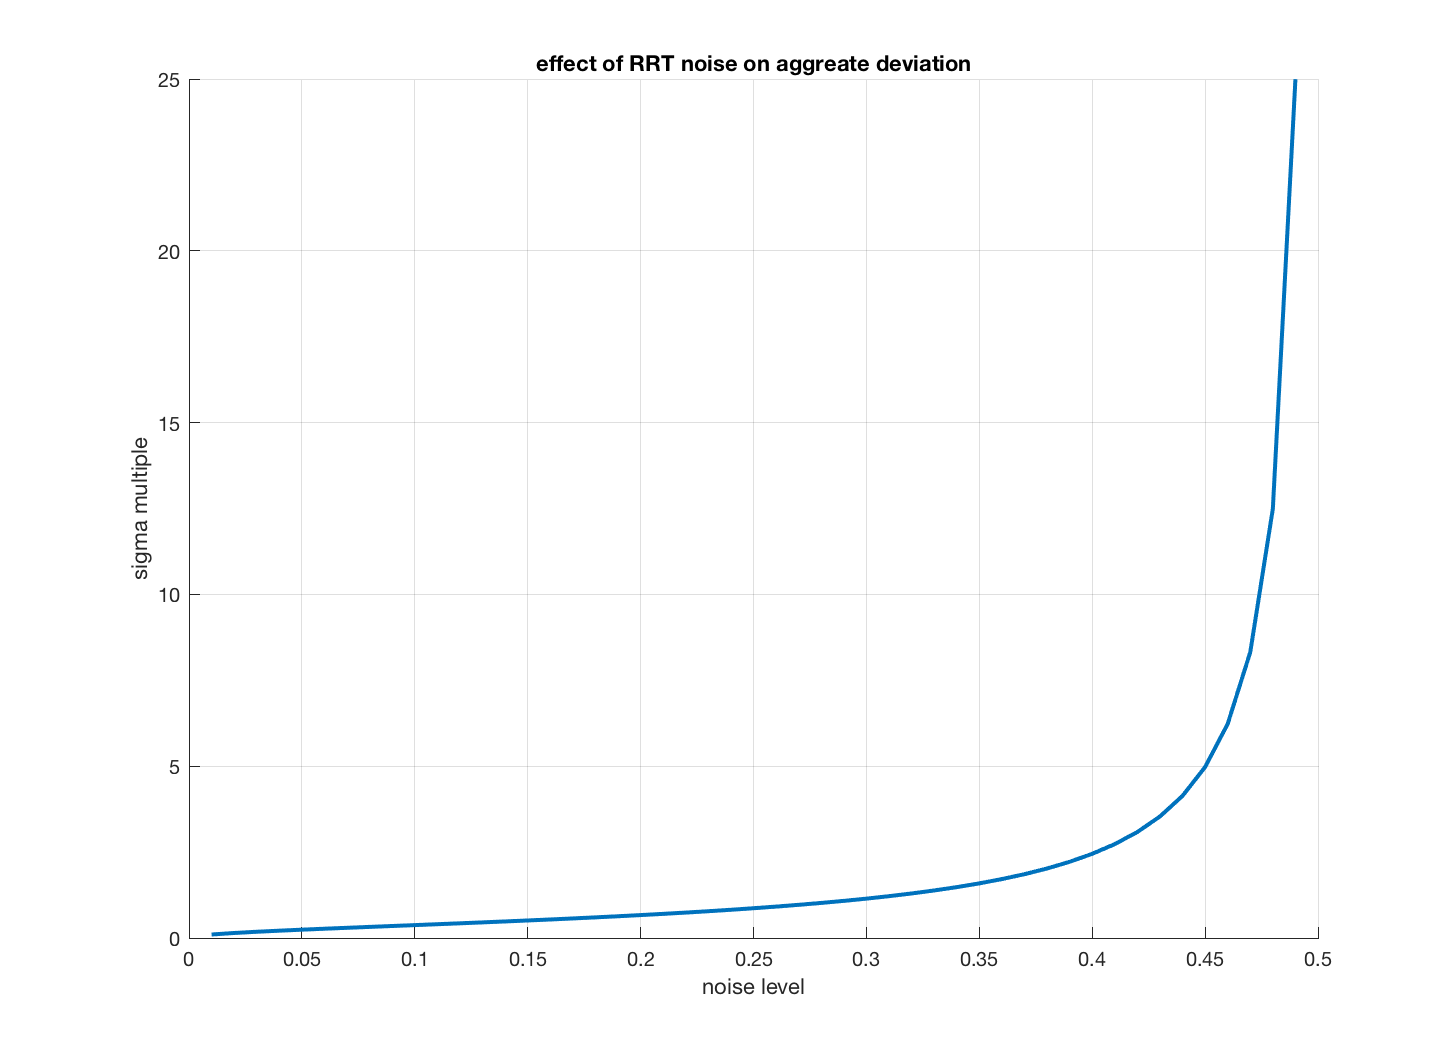
\includegraphics[scale =  0.25]{noise_effect.png}

It actually could be very significant.  Even for relatively short bit vectors of size $L=5$, the required local DP noise is:
 \begin{align}
\left ( \frac{p}{q} \right )^L \le \lambda = e^\epsilon \\
q \ge \frac{1}{1+ \lambda^{\frac{1}{L}}}
\end{align}

Using our example above for $\lambda = 2$, the local DP noise is:
 \begin{align}
q = \frac{1}{1+ \lambda^{\frac{1}{L}}}= 0.465
\end{align}

This noise level results in estimate deviation equal to $\sigma = 7.5 \sqrt{N} $.  However, if we take into account that there are $1M$  records contributing to synthetic collection and employ sufficient privacy, the corresponding noise level is only $q=0.19$ and deviation becomes $\sigma = 0.6 \sqrt{N} $.  This is $12$ fold increase in precision! 

Consider a far more radical example.  Suppose $L=40$ and $N=10M$.   This actually resembles a typical use case: $40$ bits is a sufficiently long vector to encode user data, while $10M$ users is very achievable given todays massive audiences.  For dimensionality that high  local DP may not provide useful utility.  The required noise for local DP is $q=0.4957$.  The noise that high increases deviation $58$ times!  In practical terms, it means that measured aggregates could deviate $600K$ units in either direction.  This is a very, very bad aggregation quality, unlikely to meet any business goal save the very crude estimates of very large sub-populations.

Contrast that to the precision the sufficient privacy enables.  The required noise is $q=0.4$ which multiples deviation only by $2.5$ ($22$x precision increase).  And the measurer will be able to estimate with the error not exceeding $25K$.  Which is  sufficient to estimate even 0.25\% of the population with 10\% error.  Which seems to provide utility good enough for  many practical applications.

\subsection{Laplacian noise randomization}
Here we consider user records that from continuous domains - like hight, weight, salary, etc...  A classical example for Laplacian noise application is computing an average of something, for example an salary average across company employees.  In which case, one would expect large number of modestly paid employees and only very few very high waged employees from higher management.  Collecting salary data unprotected immediately reveals CEO salary level if he chooses to donate his data.  In order to avoid exposing CEO salary, a common local DP method is to add Laplacian noise with very high deviation to every report, which makes an observer unable to tell with certainty if high salary reading belongs to a CEO or just a random noise fluctuation.  In local settings this noise is very, very high - often exceeding difference between CEO and the lowest paying employee, which indeed makes reporting extremely noise.  We show how (and how much) anonymization allows to reduce such noise.

Again we have $N$ records that take values from real valued domain.   The maximally distant pair are simply smallest and largest values we expect to find in the dataset at hand - denote them as $U_{min}$ and $U_{max}$.

The  Laplacian noise $\mathbb{L}(u_i,b)$ added to every original value $u_i$ with PDF below:
 \begin{align}
  p(x) = \frac{1}{2b}e^{-\frac{| x - u_i|}{b}}  
\end{align}
 
Computing Renyi divergence to get distributional moments of $X_1$
\begin{align}
 D_{\alpha} (X_1) =   \frac{1}{\alpha - 1} log  \left [ E \left ( \frac{p(s|u_1)^{\alpha-1}}{ p(s|u)^{\alpha-1} } \right ) \right ]  \\
 = \frac{1}{\alpha - 1} \log \int \left ( \frac{\frac{1}{2b}e^{-\frac{| x - U_{max}|}{b}}} {  \frac{1}{2b}e^{-\frac{| x - U_{min}|}{b}} } \right )^{\alpha-1}   \cdot \frac{1}{2b}e^{-\frac{| x - U_{max}|}{b}} \\
 =  \frac{1}{\alpha - 1} \log \int  \left (  e^{\frac{| x - U_{min}| - | x - U_{max}|}{b}}  \right )^{\alpha-1}   \cdot \frac{1}{2b}e^{-\frac{| x - U_{max}|}{b}}
 \end{align}

Extraction of moments of $X_1$ is done by direct integration and is lengthly, hence moved to Appendix 2.  

Below are central moments of $X_1$:
\begin{align}
 E(X_1)  \approx  \frac{2}{3}e^{\frac{U_{max} - U_{min}}{b}}  \\
  VAR(X_1)\approx  \frac{7}{45} e^{2\frac{U_{max} - U_{min}}{b}} 
 \end{align}
 
 Using these moments in the DP bound below gives the desired expression for $b$
 \begin{align}
\frac{E(X_1)}{N} + \beta \sqrt{ \frac{\var X_1}{N}} \le \lambda \\
\text{setting } \phi = e^{\frac{U_{max} - U_{min}}{b}} \\ 
 \frac{2}{3N}\phi +  \beta \sqrt{ \frac{7 \phi^2}{45 N}} \le \lambda  \\
\phi \left (   \frac{2}{3N} +   \beta \sqrt{ \frac{7}{45 N} } \right ) \le \lambda \\ 
 \frac{U_{max} - U_{min}}{b}  \le \log(\lambda) - \log \left (   \frac{2}{3N} +   \beta \sqrt{ \frac{7}{45 N} } \right )  \\
 b \ge  \frac{U_{max} - U_{min}} {  \log(\lambda) - \log \left (   \frac{2}{3N} +   \beta \sqrt{ \frac{7}{45 N} } \right ) }
 \end{align}
 
For a concrete numerical example let's come back to salary use case.  Suppose the largest salary is \$$1M$ and the smallest is $0$, $\lambda=2$, $N=100K$ and $\beta=3$.  Plugging these numbers makes $b=160,000$.   

Contrast that to local DP level on noise
 \begin{align}
 e^{\frac{U_{max} - U_{min}}{b}} \le \lambda \\
b \ge  \frac{U_{max} - U_{min}}{log(\lambda)} \\
b \ge 1,442,700
 \end{align}
 
 That's nearly 10x noise reduction, and since deviation of Laplacian noise is $\sqrt{2} b$, this is also $10x$ increase in precision.  Of cause we would like to see $100$x increase in precision, but for that we should go to the next section that discusses an intriguing technique of "fake" records.
 
\section{Appendices}
\subsection{Appendix 1}

From  \eqref{eq:outlierProbs} we have
\begin{align}
P(S|U_{N-1} \cup u_1) =  \frac{ P(S|U_N)} {N} \sum_{i=1}^N  \frac{ p(s_i | u_1) } { p(s_i | u) }
\end{align} 

Let's add another record $u'$ and condition $P(S'|U_{N-1} \cup u_1 \cup u' )$ on $u'$ generating every $s_i$ as in following:

\begin{align}
P(S'|U_{N-1} \cup u_1 \cup u' ) =  \sum_{i=1}^{N+1} p(s_i|u')  \cdot P(S' \cap s_i | U_{N-1} \cup u_1) \\
=  \sum_{i=1}^{N+1} p(s_i|u')  \cdot \left ( \frac{P(S'  \cap s_i |U_N)}{N}  \sum_{j=1, j\ne i}^{N+1} \left [ \frac{p(s_j|u_1)}{p(s_j|u)} \right ] \right  ) \\
=  \sum_{i=1}^{N+1} p(s_i|u')  \cdot \frac{p(s_i|u)}{p(s_i|u)} \cdot \frac{P(S'  \cap s_i |U_N)}{N}  \left (  \sum_{j=1, j\ne i}^{N+1} \left [ \frac{p(s_j|u_1)}{p(s_j|u)} \right ] \right  ) \\
= \sum_{i=1}^{N+1}  \frac{p(s_i|u')}{p(s_i|u)} \cdot \frac{p(s_i|u) \cdot P(S'  \cap s_i |U_N)}{N}  \left (  \sum_{j=1, j\ne i}^{N+1} \left [ \frac{p(s_j|u_1)}{p(s_j|u)} \right ] \right  ) 
\end{align} 

Note that:
\begin{align}
 p(s_i|u) \cdot P(S'  \cap s_i |U_N) = p(s_i|u) \cdot N! \prod_{j=1,j \ne i}^{N+1} p(s_j|u) = N!  \prod_{j=1}^{N+1} p(s_j|u) \\
 = \frac{N+1}{N+1} N!  \prod_{j=1}^{N+1} p(s_j|u) \\
 = \frac{(N+1)!  \prod_{j=1}^{N+1} p(s_j|u)}{N+1} \\
 =  \frac{P(S'|U_{N+1})}{(N+1)} \\
\end{align}

This allows to simplify $3.4$ as following:
\begin{align}
P(S'|U_{N_1} \cup u_1 \cup u' ) =  \frac{P(S'|U_{N+1})}{N \cdot (N+1)} \cdot  \sum_{i=1}^{N+1}  \frac{p(s_i|u')}{p(s_i|u)}\left (  \sum_{j=1, j\ne i}^{N+1} \left [ \frac{p(s_j|u_1)}{p(s_j|u)} \right ] \right  )  \\
= \frac{P(S'|U_{N+1})}{N \cdot (N+1)} \cdot  \sum_{i=1}^{N+1}  \frac{p(s_i|u')}{p(s_i|u)} \cdot \left (   \frac{p(s_i|u_1)}{ p(s_i|u) } -  \frac{p(s_i|u_1)}{ p(s_i|u) }  + \sum_{j=1, j\ne i}^{N+1} \left [ \frac{p(s_j|u_1)}{p(s_j|u)} \right ] \right  ) \\
=  \frac{P(S'|U_{N+1})}{N \cdot (N+1)} \cdot  \sum_{i=1}^{N+1}  \frac{p(s_i|u')}{p(s_i|u)} \cdot \left ( - \frac{p(s_i|u_1)}{ p(s_i|u) }  + \sum_{j=1}^{N+1} \left [ \frac{p(s_j|u_1)}{p(s_j|u)} \right ] \right  ) \\
=  \frac{P(S'|U_{N+1})}{N \cdot (N+1)} \cdot  \left (  \left [ \sum_{i=1}^{N+1}  \frac{p(s_i|u')}{p(s_i|u)} \right ] \cdot  \left [  \sum_{i=1}^{N+1}  \frac{p(s_i|u_1)}{p(s_i|u)} \right ] - \sum_{i=1}^{N+1}  \frac{p(s_i|u')}{p(s_i|u)} \cdot  \frac{p(s_i|u_1)}{p(s_i|u)} \right ) \\
\end{align} 

Restating for clarity:
 \begin{equation}  
P(S'|U_{N_1} \cup u_1 \cup u' ) =  \frac{P(S'|U_{N+1})}{N(N+1)} \cdot \left (  \left [ \sum_{i=1}^{N+1}  \frac{p(s_i|u')}{p(s_i|u)} \right ] \cdot  \left [  \sum_{i=1}^{N+1}  \frac{p(s_i|u_1)}{p(s_i|u)} \right ] - \sum_{i=1}^{N+1}  \frac{p(s_i|u')}{p(s_i|u)} \cdot  \frac{p(s_i|u_1)}{p(s_i|u)} \right )
\end{equation}

\subsection{Appendix 2}

\begin{align}
f(x) = \left\{
 \begin{matrix} 
e^{\frac{U_{min} - U_{max}}{b}}, \text{for }  x < U_{min}   \\ 
e^{\frac{2x - U_{min} - U_{max}}{b}}, \text{for }  U_{min} \le x < U_{max} \\
 e^{\frac{U_{max} -U_{min}}{b}}, \text{for }   U_{max} \le x
  \end{matrix}\right.
\end{align}

\begin{align}
E(X_1) = \int_{-\infty}^{\infty} f(x)  \frac{1 }{2b}e^{-\frac{| x - U_{max}|}{b}}  dx \\
 E(X_1) = \left\{
 \begin{matrix} 
 \int_{-\infty}^{U_{min}}   \frac{1 }{2b} e^{\frac{U_{min} - U_{max}}{b}} e^{-\frac{U_{max} - x}{b}}  dx   \text{  } + \\ 
 \int_{U_{min}}^{U_{max}}    \frac{1 }{2b} e^{\frac{2x - U_{min} - U_{max}}{b}} e^{-\frac{U_{max} - x}{b}}  dx  \text{  } + \\
  \int_{U_{max}}^{\infty}    \frac{1}{2b} e^{\frac{U_{max} -U_{min}}{b}} e^{-\frac{x - U_{max}}{b}}  dx 
  \end{matrix}\right. \\
  E(X_1) = \frac{1}{2}e^{2\frac{U_{min} - U_{max}}{b}} + \int_{U_{min}}^{U_{max}}    \frac{1 }{2b} e^{\frac{3x -  2U_{max} - U_{min}}{b}}  dx  \text{  } +  \frac{1}{2}  e^{\frac{U_{max} -U_{min}}{b}} \\
  E(X_1) = \frac{1}{2}e^{2\frac{U_{min} - U_{max}}{b}} +   \frac{1}{6}e^{\frac{U_{max} - U_{min}}{b}}   -   \frac{1}{6}e^{2\frac{U_{min} - U_{max}}{b}}   +  \frac{1}{2}  e^{\frac{U_{max} -U_{min}}{b}} \\
  E(X_1)  \approx  \frac{2}{3}e^{\frac{U_{max} - U_{min}}{b}}  
\end{align}

\begin{align}
E(X^2_1) = \int_{-\infty}^{\infty} f^2(x)  \frac{1 }{2b}e^{-\frac{| x - U_{max}|}{b}}  dx \\
 E(X^2_1) = \left\{
 \begin{matrix} 
 \frac{1}{2}e^{3\frac{U_{min} - U_{max}}{b}}   \text{  } + \\ 
 \int_{U_{min}}^{U_{max}}    \frac{1 }{2b} e^{\frac{5x -  3U_{max} - 2U_{min}}{b}}  dx  \text{  } + \\
 \frac{1}{2}e^{2\frac{U_{max} - U_{min}}{b}}
  \end{matrix}\right. \\
   E(X^2_1) =   \frac{1}{2}e^{3\frac{U_{min} - U_{max}}{b}}  +  \frac{1}{10}e^{2\frac{U_{max} - U_{min}}{b}}   -   \frac{1}{10}e^{3\frac{U_{min} - U_{max}}{b}}   +  \frac{1}{2}e^{2\frac{U_{max} - U_{min}}{b}}\\
  E(X^2_1) \approx   \frac{3}{5}e^{2\frac{U_{max} - U_{min}}{b}} \\
  VAR(X_1) = X^2_1 - E(X_1)^2 \approx  \frac{3}{5}e^{2\frac{U_{max} - U_{min}}{b}} -  \frac{4}{9}e^{2\frac{U_{max} - U_{min}}{b}} =  \frac{7}{45} e^{2\frac{U_{max} - U_{min}}{b}} 
\end{align}


\end{document}

